    Concurrent programs take advantage of \textit{out-of-order} execution. Intuitively, this means that more than one unrelated computations can be done ``simultaneously'' without having any fixed order in which they should happen. 
    This results in concurrent programs having multiple different outcomes, the possible outcomes of which are described by
    a \textit{memory consistency model}. 
    The most intuitive and commonly relied upon model is that of \textit{Sequential Consistency} (SC), which guarantees that every outcome of a program must be equivalent to a sequential interleaving of each thread's individual actions. 
    For example, consider the program in Figure~\ref{intro:Example} with two threads, which share memory denoted by $x$, $y$ initialized to 0, where $a$, $b$ are local variables. The right-hand-side are the possible values that $a$ and $b$ can read under sequential consistency rules.
    
    %Show program 
    \begin{figure}[H]
        \centering
        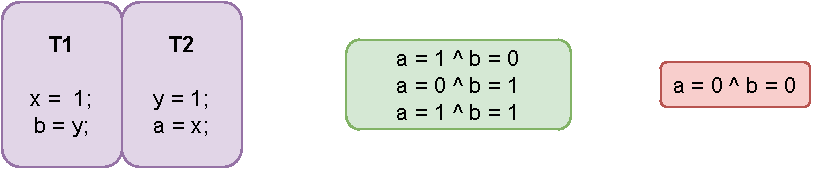
\includegraphics[scale=0.7]{1.Introduction/SC_Example1(a).pdf}
        \caption{Example program with its possible outcomes under sequential consistency.}
        \label{intro:Example}
    \end{figure}
    
    
    However, the above program under SC cannot have the outcome $a=0\ \wedge\ b=0$ as given in the red box to the right. To show that it is indeed not possible, assume that $a=0$. This means $x=1$ has not been done while $y=1$ has been done. This also means $b=y$ has not been done yet. Hence, if now the read to $y$ occurs, it cannot be $0$. The case is similar for when $b=0$. 
    Such sequential reasoning though easy to understand and follow while writing concurrent programs, may not be that advantageous from a performance perspective.  
    From a program transformation standpoint, the above disallowed outcome should be possible: we can simply reorder either the two events in $T1$ or that in $T2$ as they are disjoint memory operations. 
    But from a sequential consistency standpoint, since the outcome is not valid, it also brings with it the question whether such simple program transformations are even valid to perform.
    Figure~\ref{intro:Example2} shows how after doing either one of these reorderings, an outcome invalid under SC is possible. 
    %Show program 
    \begin{figure}[H]
        \centering
        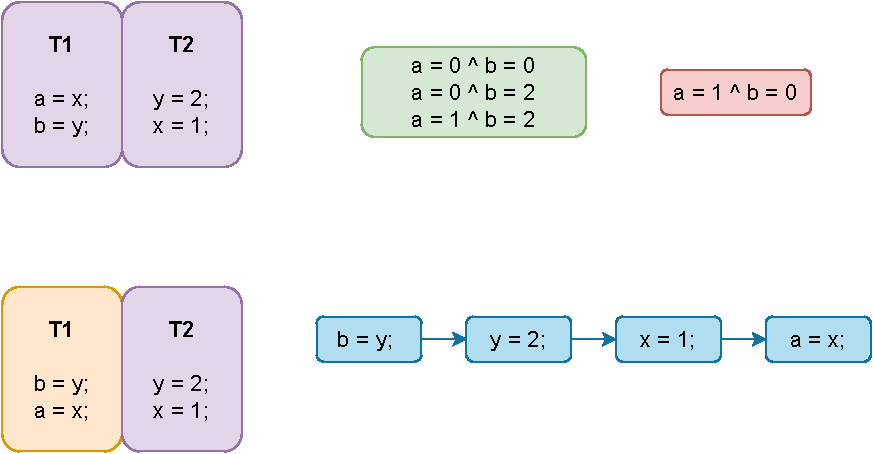
\includegraphics[scale=0.7]{1.Introduction/SC_Example1(b).pdf}
        \caption{The original program above with its allowed and disallowed outcomes in SC, followed by the program with the two reads reordered below, justifying the disallowed outcome under SC.}
        \label{intro:Example2}
    \end{figure}

    The reordered program can justify a sequential interleaving of events to have the disallowed outcome in the original program. 

    Such concerns are not only related to simple reordering, but also something such as elimination. 
    Yet another example can be that of elimination. Consider the program in Figure \ref{intro:Example3} below
    \begin{figure}[H]
        \centering
        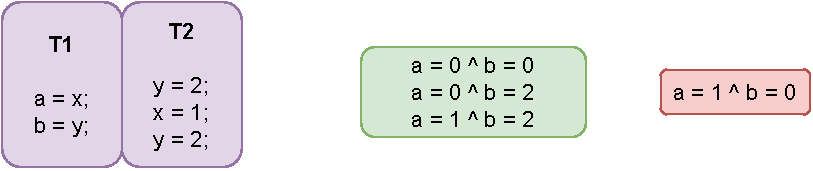
\includegraphics[scale=0.7]{1.Introduction/SC_Example2(a).pdf}
        \caption{Another program above with its allowed and disallowed outcomes under SC.}
        \label{intro:Example3(a)}
    \end{figure}

    In this example, the red box outcome is still not allowed under SC. We can notice though that the write to $y$ in $T2$ is done twice. 
    Naturally, the compiler might think of eliminating one of them under the context of redundant code elimination. 
    Suppose it eliminates the first write $y=2$. 
    Then the resulting program as shown below in Figure \ref{intro:Example3(b)}, can justify the outcome under SC whcih was disallowed in the original program.
    \begin{figure}[H]
        \centering
        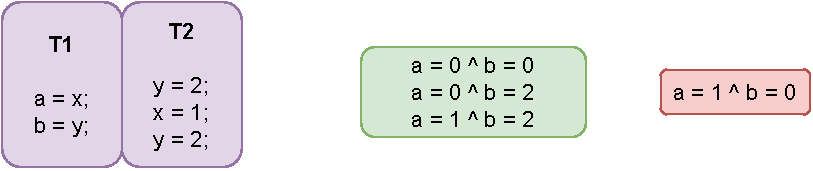
\includegraphics[scale=0.7]{1.Introduction/SC_Example2(a).pdf}
        \caption{Program after elimination of $y=2$, justifying disallowed outcome under SC.}
        \label{intro:Example3(b)}
    \end{figure}

    The above examples show that even simple transformations can be unsound under SC. Complex program transformations such as register allocation, common-sub-expression elimination, loop invariant code motion are some examples which use the above two basic transformations heavily. 
    Having them unsound under SC also implies the compiler is not allowed to do a varying class of optimization without breaking the consistency rules udner which the concurrent program is supposed to behave / execute. 

    In addition, the performance of programs executing under SC, but coupled with program transformations, many of which are disallowed in most programs without locks, did not seem to be an effective choice for programming. 
    In addition, hardware at that time had come up with several features such as buffers and cache systems, which in principle could be used effectively for performance, but were not so useful for programs respective SC semantics. 
      
    For this reason, weaker consistency models have been introduced to concurrent, shared-memory languages (both high and low level) to leverage more of the \textit{out-of-order} execution notion. 
    For instance, under the ECMAScript consistency model semantics, if all the accesses are of type \textit{unordered}, the above invalid outcome is allowed, which implies a reordering of such events is valid in the above case. 
    The problem, however, is that semantics of such weak consistency can be easily misunderstood, and is often defined in informal prose format, thus leading to misinterpretation of intended semantics, which leads to several issues. 
    Other problems that exist is incorrect compilation, which causes programs to misbehave when executed on different hardware / target lanaguegs. 
    It has also been shown that verification of such programs is much difficult to do due to more state space explosions.
    For our purpose, it makes it difficult to assert when a particular program transformation is valid / safe. 
    
    Our focus, therefore, in this thesis is to first offer a clarified, more concise rendition of the core ECMAScript memory model that allows for better abstract reasoning over allowed and disallowed behaviours (outcomes). 
    We use our model to provide a straightforward, conservative proof of when reordering of independent instructions and elimination is permitted, addressing optimization in terms of its impact on observable program behaviours. 
    Specific contributions of our work include the following:
    
    \begin{enumerate}
        \item We provide a concise \textit{declarative(axiomatic) style} model of the core ECMAScript memory consistency semantics. This clarifies the existing draft presentation~\cite{ECMA} in a manner useful for validating optimizations.
        \item Using this model, we show when basic reordering of independent instructions is allowed. We extend this to reordering in the presence of conditionals and loops in programs.
        \item Similar proof designs are used to validate other basic optimization behaviours such as removing redundant reads or writes. Further extending it to elimination in the presence of conditionals and loops. 
        \item We lastly show how our above two results help us check the validity of loop invariant code motion. 
    \end{enumerate}
  